\documentclass{beamer}
\usepackage[utf8]{inputenc}
% \usepackage[T1]{fontenc}
% \usepackage[english]{babel}
\usepackage{wrapfig}
\usepackage{verbatim}
\usepackage{ mathrsfs }
\usepackage{dsfont}
\usepackage{amssymb}
\usepackage{amsmath}
\usepackage{amsthm}
\usepackage{graphicx}
\usepackage{lmodern}
\usepackage{float}
\usepackage{listings}
\usepackage{hyperref}
\usepackage{array}
\usepackage{multirow}
\usepackage{caption}
\usepackage{subcaption}
\usepackage{tikz}
\usepackage{tikzsymbols}
\usetikzlibrary{positioning} 
\usetheme{Madrid}
\DeclareMathOperator*{\argmin}{argmin}
\DeclareMathOperator*{\argmax}{argmax}

\title{Inferring the underlying network of diffusion}

\begin{document}
\begin{frame}
\titlepage
\begin{figure}
    \centering
    
\includegraphics[scale = 0.5]{EPFL_Todai.jpg}
\end{figure}
\begin{tabular}{l}
     Supervisors :  \\
     Prof. Friedrich Eisenbrand\\
     Prof. Iwata Satoru\\
     Dr. Tasuku Soma
\end{tabular}
\hfill
\begin{tabular}{l}
     Student : \\
     Joachim Moussalli
\end{tabular}
\end{frame}

\begin{frame}{Table of Contents}
\tableofcontents
\end{frame}
\section{Introduction}
\begin{frame}{Motivation}
\begin{columns}
\column{0.5\textwidth}
(Fake) News
\column{0.5\textwidth}
\begin{figure}
    \centering
    
\includegraphics[scale = 0.1]{FakeNews.jpg}
\end{figure}
\end{columns}

\begin{columns}
\column{0.5\textwidth}
Marketing
\column{0.5\textwidth}
\begin{figure}
    \centering
    
\includegraphics[scale = 0.1]{Iphone.jpg}
\end{figure}
\end{columns}

\begin{columns}
\column{0.5\textwidth}
Diseases
\column{0.5\textwidth}
\begin{figure}
    \centering
    
\includegraphics[scale = 0.1]{diseases.jpg}
\end{figure}
\end{columns}
\end{frame}
\begin{frame}{Problem- Underlying network}
\begin{figure}
\begin{subfigure}{.4\textwidth}
    \centering
    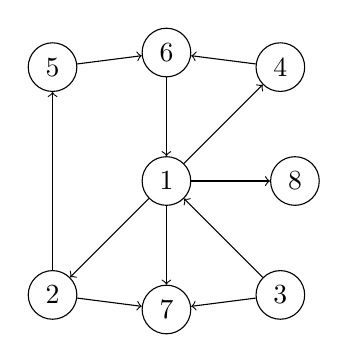
\begin{tikzpicture}[roundnode/.style = {circle, draw=black}]
     \node[roundnode] (1) {1};
     \node[roundnode] (2) [below left=of 1]{2};
     \node[roundnode] (3) [below right=of 1]{3};
     \node[roundnode] (5) [above left=of 1]{5};
     \node[roundnode] (4) [above right=of 1]{4};
     \node[roundnode] (6) [above=of 1]{6};
     \node[roundnode] (7) [below=of 1]{7};
     \node[roundnode] (8) [right=of 1]{8};
     
     \draw[->] (1)--(2);
     \draw[->] (1)--(4);
     \draw[->] (1)--(7);
     \draw[->] (1)--(8);
     \draw[->] (2)--(5);
     \draw[->] (2)--(7);
     \draw[->] (3)--(1);
     \draw[->] (3)--(7);
     \draw[->] (4)--(6);
     \draw[->] (5)--(6);
     \draw[->] (6)--(1);
\end{tikzpicture}
\caption{Unkown underlying network,$G^* = (V,E^*)$}
\end{subfigure}
\begin{subfigure}{.4\textwidth}
    \centering
    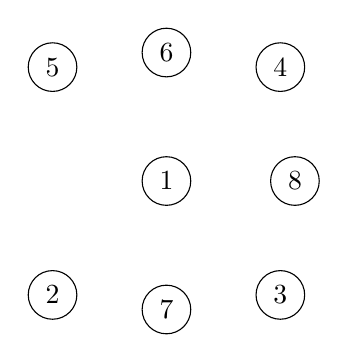
\begin{tikzpicture}[roundnode/.style = {circle, draw=black}]
     \node[roundnode] (1) {1};
     \node[roundnode] (2) [below left=of 1]{2};
     \node[roundnode] (3) [below right=of 1]{3};
     \node[roundnode] (5) [above left=of 1]{5};
     \node[roundnode] (4) [above right=of 1]{4};
     \node[roundnode] (6) [above=of 1]{6};
     \node[roundnode] (7) [below=of 1]{7};
     \node[roundnode] (8) [right=of 1]{8};
\end{tikzpicture}
\caption{Find the edges.}
\end{subfigure}
\end{figure}
\end{frame}
\begin{frame}{Problem- Independent cascades model}
\begin{block}{Propagation Rules}
\begin{itemize}
    \item The infection is observed during a time window of length T (T = 6).
    \item The time of infection of a vertex $i$ is determined by $t_i = \min_{j \in N^+(i)} t_j + \Delta t_{j,i}$. Where $\Delta t_{i,j} {\sim} Exp(\alpha)$ 
\end{itemize}
\end{block}
\begin{figure}
\begin{subfigure}{.4\textwidth}
    \centering
    \begin{tikzpicture}[roundnode/.style = {circle, draw=black}, infectednode/.style = {circle, draw=black, fill = green}, toolate/.style = {circle, draw = black, fill = red}]
     \node[roundnode] (1) {1};
     \only<4->\node[infectednode, label = 180:2.0] (1) {1};
     \only<1-4>\node[roundnode] (2) [below left=of 1]{2};
     \only<5-> \node[infectednode, label = 180:3.2] (2) [below left=of 1]{2};
     \node[roundnode] (3) [below right=of 1]{3};
     \only<1>\node[roundnode] (5) [above left=of 1]{5};
     \only<2->\node[infectednode, label = 0] (5) [above left=of 1]{5};
     \node[roundnode] (4) [above right=of 1]{4};
     \only<6->\node[infectednode, label = 3.4] (4) [above right=of 1]{4};
     \node[roundnode] (6) [above=of 1]{6};
     \only<3->\node[infectednode, label = 0.9] (6) [above=of 1]{6};
     \node[roundnode] (7) [below=of 1]{7};
     \only<7->\node[infectednode, label = -90:5.8] (7) [below =of 1] {7};
     \node[roundnode] (8) [right=of 1]{8};
     \only<8-> \node[toolate, label = 7.1] (8) [right = of 1] {8};
     \draw[->] (1)--(2);
     \only<5->\draw[thick,->] (1)--(2);
     \draw[->] (1)--(4);
     \only<6->\draw[thick,->](1)--(4);
     \draw[->](1)--(7);
     \only<1-7>\draw[->](1)--(8);
     \only<8-> \draw[dotted,->] (1)--(8);
     \draw[->] (2)--(5);
     \draw[->] (2)--(7);
     \only<7-> \draw[thick,->] (2)--(7);
     \draw[->] (3)--(1);
     \draw[->] (3)--(7);
     \draw[->] (4)--(6);
     \draw[->] (5)--(6);
     \only<3->\draw[thick,->] (5)--(6);
     \draw[->] (6)--(1);
     \only<4->\draw[thick,->] (6)--(1);
\end{tikzpicture}
\end{subfigure}
\begin{subfigure}{.4\textwidth}
    \centering
    \begin{tikzpicture}[roundnode/.style = {circle, draw=black}, infectednode/.style = {circle, draw=black, fill = green}]
     \node[roundnode] (1) {1};
     \only<4->\node[infectednode] (1) {1};
     \node[roundnode] (2) [below left=of 1]{2};
     \only<5-> \node[infectednode] (2) [below left=of 1]{2};
     \node[roundnode] (3) [below right=of 1]{3};
     \only<1>\node[roundnode] (5) [above left=of 1]{5};
     \only<2->\node[infectednode] (5) [above left=of 1]{5};
     \node[roundnode] (4) [above right=of 1]{4};
     \only<6->\node[infectednode] (4) [above right=of 1]{4};
     \node[roundnode] (6) [above=of 1]{6};
     \node[roundnode] (7) [below = of 1]{7};
     \only<7-> \node[infectednode] (7) [below = of 1] {7};
     \node[roundnode] (8) [right =of 1] {8};
     \only<3->\node[infectednode] (6) [above=of 1]{6};
     \only<8-> \draw[->] (5)--(6);
     \only<8-> \draw[->] (5)--(1);
     \only<8-> \draw[->] (6)--(2);
     \only<8-> \draw[->] (2)--(0,-1)--(4);
     \only<8-> \draw[->] (1)--(7);
\end{tikzpicture}
\end{subfigure}
\end{figure}
\end{frame}
\begin{frame}{Problem formulation- Infectious rates}
\begin{block}{Definition}
To each pair of vertices $(i,j)$ a weight, $\alpha_{i,j} \geq 0$, corresponding to the infectious rate is associated. Let us denote the set of infectious rate by $\mathscr{A} = \{\alpha_{i,j}|(i,j)\in V \times V, i\neq j\}.$
\end{block}
\begin{block}{Remark}
\begin{itemize}
    \item There is an edge between node $i$ and node $j$ $\iff \alpha_{i,j} > 0$.
    \item The infectious parameter might be dynamic with respect to time, i.e $\alpha_{i,j} \leadsto \alpha_{i,j}(t)$.
    \item If $\Delta t{\sim} Exp(\alpha)$ then $E[\Delta t]=\frac{1}{\alpha}$. It is the \textit{expected waiting time}.
\end{itemize}
\end{block}
\end{frame}

\begin{frame}{Example}
\begin{columns}
\column{0.5\textwidth}
\begin{figure}
    \centering
    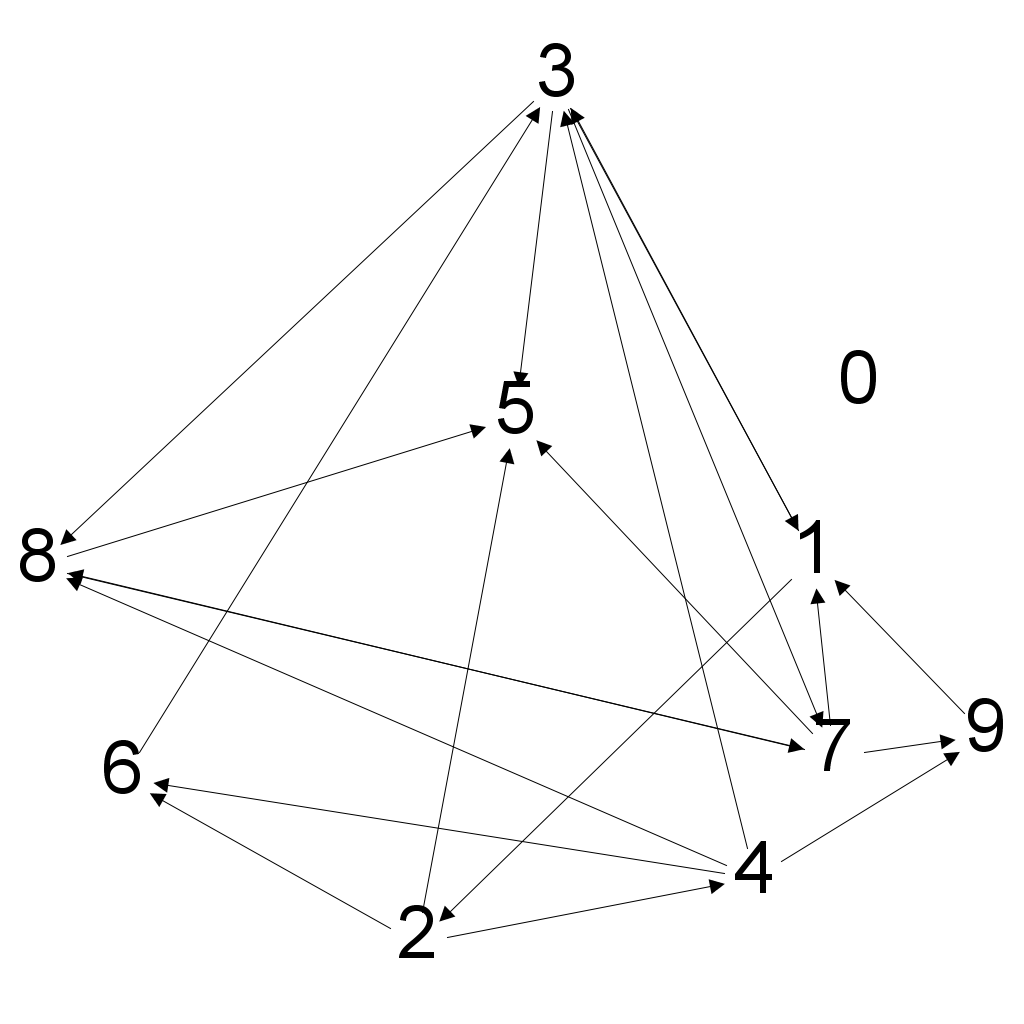
\includegraphics[scale = 0.1]{G_star.png}
    \caption{Inferred Network $\hat{G} = (10,21)$ with $MSE = 0.015$.}
\end{figure}
\column{0.5\textwidth}
\begin{figure}
    \centering
    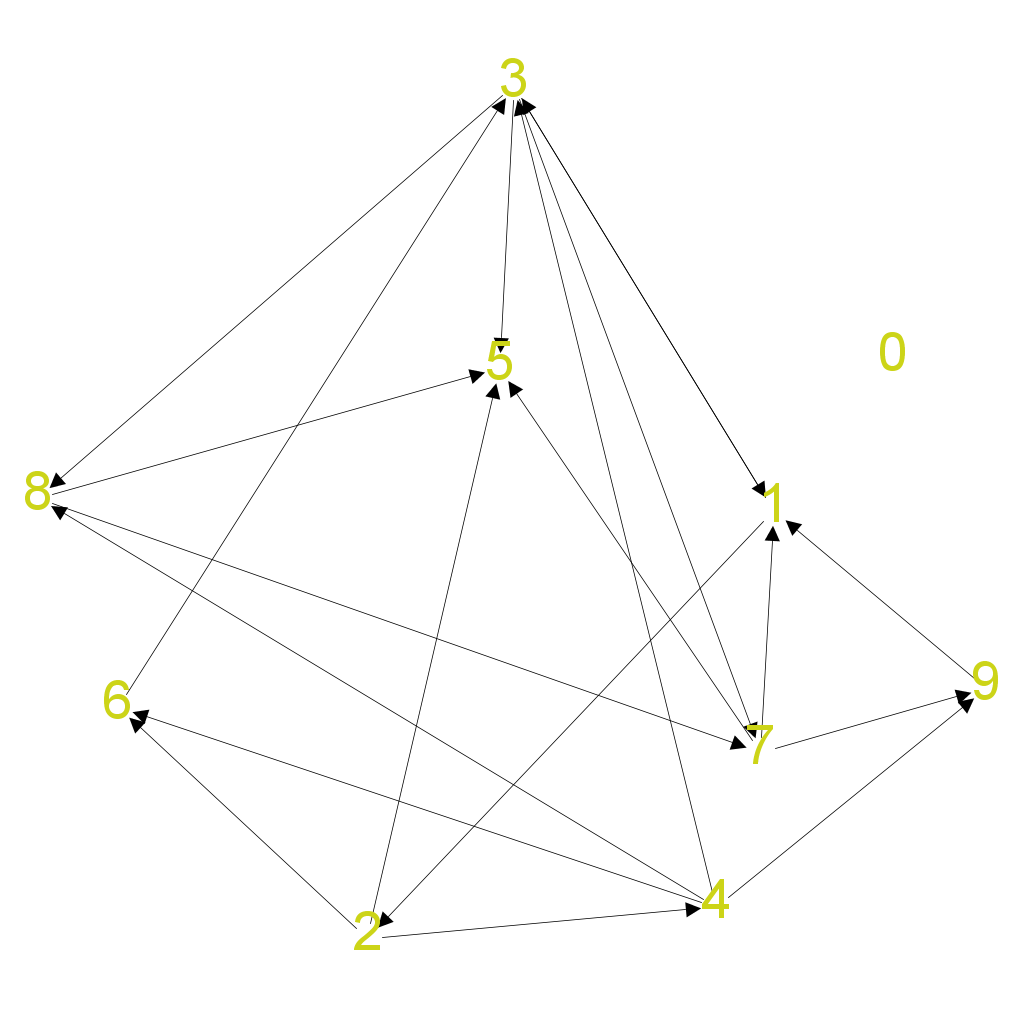
\includegraphics[scale = 0.1]{G-true2.png}
    \caption{True network $G^* = (10,20)$ with $|C| = 100$ cascades.}
\end{figure}
\end{columns}
\end{frame}
\begin{frame}{Problem formulation}
\begin{block}{Problem 1- Discrete optimization (edge vs no-edge)}
Given a collection of cascade $C$ propagating over a set of vertices $V$, find the underlying network $G^*$.
\end{block}
\begin{block}{Problem 2- Continuous optimization (who is $\alpha$ ?)}
Given a collection of cascade $C$, find the correct infection parameters set $\mathscr{A}$.  
\end{block}
\begin{figure}
    \centering
    
\includegraphics[scale = 0.08]{Detective_Pikachu_-_Character_artwork_01.png}
\end{figure}
\end{frame}

\section{Related work}
\begin{frame}{Related work}
\begin{block}{Solutions of Problem 1 (edge vs no-edge)}
\begin{itemize}
    \item {[Gomez-Rodriguez,Leskovec and Krause,'12]}\nocite{NetInf} and [Gomez-Rodriguez and Schölkopf,'12] \nocite{MultiTrees} developed \textit{NetInf} and \textit{MultiTrees} algorithms.
    \item Submodular optimization with greedy algorithm.
    \item Requires apriori knowledge of the number of edges.
    \item Hard/Not efficient to extend to the dynamic setting.
\end{itemize}
\end{block}
\end{frame}
\begin{frame}{Related work}
\begin{block}{Solution of Problem 2 (who is $\alpha$ ? )}
\begin{itemize}
    \item {[G-R,Balduzzi and Scholkopf,'11]}\nocite{NetRate} and [G-R,Leskovec and Scholkopf,'12]\nocite{InfoPath} developed \textit{NetRate} and \textit{InfoPaths} algorithms.
    \item Convex optimization solved with CVX and stochastic gradient descent (SGD).
    \item Easily extendable to the dynamic setting and no apriori knowledge needed.
    \item Computation time is higher than NetInf.
    \item No convergence complexity proofs.
\end{itemize}
\end{block}
\end{frame}
% \begin{frame}{Probabilistic modeling (Exponential case)}
% \begin{itemize}
%     \item \textbf{Likelihood of transmission} $j\rightarrow i$ : %ATTENTION : Does not mean that j is the FIRST to infect i.
%     \begin{equation}
%     \mathscr{L}(\alpha_{j,i}|t_i-t_j) = f_{\alpha_{j,i}}(t_i-t_j) = \begin{cases}
%     \alpha_{j,i} e^{-\alpha_{j,i}(t_i-t_j)}     &  \text{if} t_j < t_i\\
%     0    & \text{otherwise}
%     \end{cases}
% \end{equation}
% \item \textbf{Cumulative density function (CDF)} :
% \begin{equation}
%     F(t_i-t_j;\alpha_{j,i}) = \int_{0}^{t_i-t_j}f_{\alpha_{j,i}}(t)dt = 1-e^{-\alpha_{j,i}(t_i-t_j)}
% \end{equation}
% \item \textbf{Survival function} of node $i$ by time $t_i$ (w.r.t node $j$):
% \begin{equation}
%     S(t_i-t_j;\alpha_{j,i})=\mathds{P}(t_j + X \geq t_i) = 1-F(t_i-t_j;\alpha_{j,i}) = e^{-\alpha_{j,i}(t_i-t_j)}
% \end{equation}
% \item \textbf{Instantaneous infection rate} :
% \begin{equation}
%     H(t_i|t_j;\alpha_{j,i}) = \frac{f_{\alpha_{j,i}}(t_i-t_j)}{S(t_i-t_j;\alpha_{j,i})} = \alpha_{j,i}
% \end{equation}
% \end{itemize}
% \end{frame}

% \begin{frame}{Likelihood of an edge in a cascade}
% \begin{block}{likelihood of an edge (j,i)}
% A node gets infected once the \alert{first} parent infects it. The likelihood of parent j being the first parent of i is given by :
% \begin{equation}
%     f_{\alpha_{j,i}}(t_i-t_j) \prod_{j\neq k,t_k<t_i}S(t_i-t_k;\alpha_{k,i})
% \end{equation}
% Then the likelihood of node i getting infected at time $t_i$ by one of the previously infected nodes $(t_1,\dots,t_N|t_k<t_i)$ is given by :
% \begin{equation}
%     \sum_{j:t_j<t_i}f_{\alpha_{j,i}}(t_i-t_j)\prod_{j\neq k,t_k<t_i}S(t_i-t_k;\alpha_{k,i})
% \end{equation}
% \end{block}
% \end{frame}
% \begin{frame}{Likelihood of a cascade}
% \begin{block}{Infected nodes}
% $\textbf{t}^{\leq T} = \{t_1,\dots,t_N|t_i\leq T\}$
%     \begin{equation}
%         \begin{split}
%             \mathscr{L}(\mathbf{t}^{\leq T};\mathscr{A}) &= \prod_{i:t_i \leq T}\sum_{j:t_j<t_i}f_{\alpha_{j,i}}(t_i-t_j)\prod_{j\neq k,t_k<t_i}S(t_i-t_k;\alpha_{k,i})\\
%             &= \prod_{i : t_i\leq T}\prod_{k:t_k<t_i}S(t_i-t_k;\alpha_{k,i}) \sum_{j:t_j<t_i}\frac{f_{\alpha_{j,i}}(t_i-t_j)}{S(t_i-t_j;\alpha_{j,i})}
%         \end{split}
%     \end{equation}
% \end{block}
% \begin{block}{Total likelihood}
% \begin{equation}
%     \mathscr{L}(\textbf{t};\mathscr{A}) = \mathscr{L}(\textbf{t}^{\leq T};\mathscr{A}) \prod_{i:t_i\leq T}\prod_{m:t_m>T}S(T-t_i;\alpha_{i,m})
% \end{equation}
% Considering a finite collection of cascade $C = \{\textbf{t}^1,\textbf{t}^2,\dots\}$, the likelihood of the infectious parameters is given by $\prod_{c \in C}\mathscr{L}(\textbf{t}^c;\mathscr{A})$
% \end{block}
% \end{frame}
\begin{frame}{Inference problem}
    \begin{block}{Problem}
    Find the transmission rates $\alpha_{i,j} \in \mathscr{A}$ for every pair of nodes such that the likelihood is maximized.
    \begin{equation}
    \begin{split}
        &\min_{\mathscr{A}} -\sum_{c\in C}\log \mathscr{L}(\textbf{t}^c;\mathscr{A})\\
        &\text{s.t  } \alpha_{i,j}\geq 0, i,j = 1,\dots,N, i\neq j
    \end{split}
    \end{equation}
    \end{block}
            $-\sum_{c\in C}\log \mathscr{L}(\textbf{t}^c;\mathscr{A}) =\sum_{c \in C}\Psi_1(\textbf{t}^c;\mathscr{A})+\Psi_2(\textbf{t}^c;\mathscr{A})+\Psi_3(\textbf{t}^c;\mathscr{A})$
\end{frame}
\begin{frame}{Properties of the minimization problem}
\begin{block}{Contribution to the objective function}
Penalize edges going to healthy nodes \begin{equation*}
    \Psi_1(\textbf{t}^c;\mathscr{A}) = \sum_{i:t_i\leq T}\sum_{m : t_m>T} \alpha_{i,m}(T-t_i)
\end{equation*}
Penalize slow infection time \begin{equation*}
    \Psi_2(\textbf{t}^c;\mathscr{A}) = \sum_{i:t_i\leq T}\sum_{j : t_j<t_i} \alpha_{j,i}(t_i-t_j)
\end{equation*}
Force infected nodes to have a parent :
\begin{equation*}
    \Psi_3(\textbf{t}^c;\mathscr{A}) = \sum_{i:t_i\leq T}-\log(\sum_{j:t_j<t_i}\alpha_{j,i})
\end{equation*}
\end{block}
\end{frame}
% \begin{frame}{Extension to the dynamic setting}
%     \begin{block}{few modifications}
%     \begin{enumerate}
%         \item $\mathscr{A}\leadsto \mathscr{A}(t) = \{\alpha_{i,j}(t)|\alpha_{i,j}\geq 0 , t\leq T\}$
%         \item $C = \{C_{T_1},C_{T_2},\dots \}$ where $C_{T_i}$ is the set of all cascades that finished before $T_i$.
%     \end{enumerate}
%     \end{block}
%     \begin{figure}
%         \centering
%         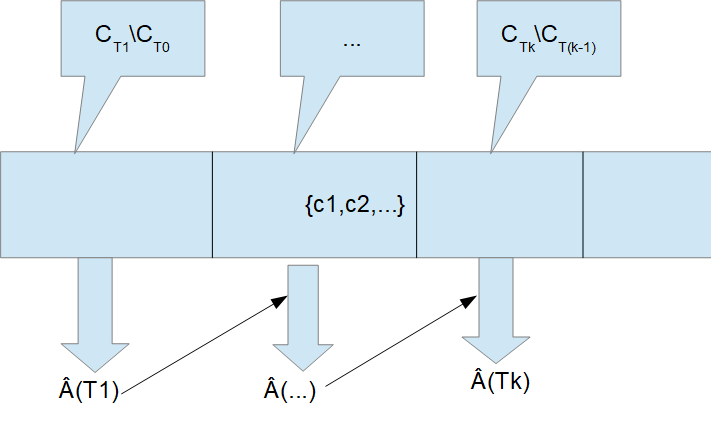
\includegraphics[scale = 0.4]{NR_dyn.png}
%     \end{figure}
% \end{frame}
\section{New algorithm}
\begin{frame}{Solving using ADMM}
    \begin{block}{ADMM for node i}
    Let $g_1(\textbf{t}^c;\Vec{\alpha_i}) = \sum_{j:t_j \leq T} \alpha_{j,i}(T-t_j) + \sum_{j : t_j<t_i} \alpha_{j,i}(t_i-t_j)$ and $g_2(\textbf{t}^c;z) = \log z $. The optimization problem reads now :
    \begin{equation}
        \begin{split}
            &\min_{\mathscr{A},z} \sum_{c\in C}g_1(\textbf{t}^c;\Vec{\alpha_i}) -  g_2(\textbf{t}^c;z)\\
            &\text{s.t } z_c = \sum_{j:t_j<t_i}\alpha_{j,i} = M_c \alpha_i, \alpha_{k,i} \geq 0 \forall k\in V.
        \end{split}
    \end{equation}
    \end{block}
    \begin{block}{Augmented Lagrangian}
    \begin{equation}
        L_\beta(\alpha_i,z,\lambda) = g_1(\textbf{t}^c;\Vec{\alpha_i}) + g_2(\textbf{t}^c;z) + \lambda(M_c \alpha_i - z_c) + \beta/2||M_c\alpha_i -z_c||^2_2
    \end{equation}
    \end{block}
\end{frame}

\begin{frame}{ADMM iteration}
    \begin{block}{Iteration}
    % \begin{equation}
    %     \begin{split}
    %         &\alpha_i^k = \min_{\alpha_i} -\sum_{c\in C} g_1(\textbf{t}^c;\Vec{\alpha_i}) + \lambda^{k-1}(M_c \alpha_i) + \beta/2 ||M_c\alpha_i - z_c^{k-1}||^2_2\\
    %         &z^k = \min_z -\sum_{c\in C} g_2(\textbf{t}^c;z) - \lambda^{k-1} z_c + \beta/2 ||M_c \alpha_i^k -z_c||_2^2\\
    %         &\lambda^k = \lambda^k + \beta(M\alpha_i^k - z^k)
    %     \end{split}
    % \end{equation}
    Update $\alpha_i ^k \leadsto$ Use GD\\
    Update $z^k \leadsto $ Close form formula\\
    Update $\lambda^k \leadsto $ Gradient ascent 
   \end{block}
    \begin{block}{Remark}
    Under the assumption that $g_1$ and $g_2$ are convex functions then, according to [He and Yuan,'11]\nocite{ADMM_Convergence}, ADMM converge in $O(1/t)$.
    \end{block}
\end{frame}
\section{Results}
\begin{frame}{Measurements tools}
    \begin{block}{Precision,Recall,Accuracy}
    Let $G^*=(V,E^*)$ be the true network and $\hat{G} = (V, \hat{E})$ be the inferred network.\\
    Precision : \begin{equation*}
        P := \frac{|\hat{E}\cap E^*|}{|\hat{E}|}
    \end{equation*}
    Recall :\begin{equation*}
        R := \frac{|\hat{E} \cap E^*|}{|E^*|}
    \end{equation*}
    Accuracy : \begin{equation*}
        A := 1-\frac{|E^*\setminus E|+|E\setminus E^*|}{|E|+|E^*|}
    \end{equation*}
    \end{block}
\end{frame}
\begin{frame}{Results}
 % Please add the following required packages to your document preamble:
% \usepackage{multirow}
\begin{table}[scale = 0.5]
\begin{tabular}{|l|l|l|l|l|l|l|}
\hline
\textbf{Graphs} & \textbf{Algos} & \textbf{Precision} & \textbf{Recall} & \textbf{Accuracy} & \textbf{MSE} & \textbf{Time} \\ \hline
\multirow{4}{*}{\textbf{(500,1k)}} & \textbf{NF} & 85 & 85 & 85 & - & 384 \\ \cline{2-7} 
 & \textbf{CVX} & 89 & 94 & 91 & 24.5 & 2192 \\ \cline{2-7} 
 & \textbf{SGD} & 84 & 93 & 88 & 0.05 & 818 \\ \cline{2-7} 
 & \textbf{ADMM} & 88 & 92 & 90 & 0.03 & 954 \\ \hline
\multirow{4}{*}{\textbf{(800,800)}} & \textbf{NF} & 81 & 81 & 81 & - & 11 \\ \cline{2-7} 
 & \textbf{CVX} & 83 & 86 & 84 & 5.28 & 593 \\ \cline{2-7} 
 & \textbf{SGD} & 67 & 88 & 76 & 0.18 & 112 \\ \cline{2-7} 
 & \textbf{ADMM} & 83 & 83 & 83 & 0.13 & 257 \\ \hline
\multirow{4}{*}{\textbf{(1k,1k)}} & \textbf{NF} & 74 & 74 & 74 & - & 10 \\ \cline{2-7} 
 & \textbf{CVX} & 81 & 82 & 81 & 19 & 898 \\ \cline{2-7} 
 & \textbf{SGD} & 67 & 85 & 75 & 0.19 & 128 \\ \cline{2-7} 
 & \textbf{ADMM} & 81 & 80 & 80 & 0.15 & 327 \\ \hline
\end{tabular}
\end{table}
\end{frame}
\begin{frame}{Results}
\begin{columns}
\column{0.5\textwidth}
\begin{figure}
    \centering
    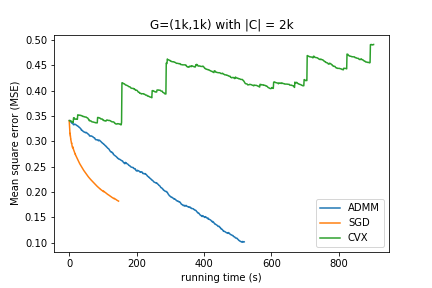
\includegraphics[scale = 0.3]{MSE_TIME_1k_1K_2k.png}
    \caption{Mean square error of ADMM, SGD and CVX}
\end{figure}
\column{0.5\textwidth}
\begin{figure}
    \centering
    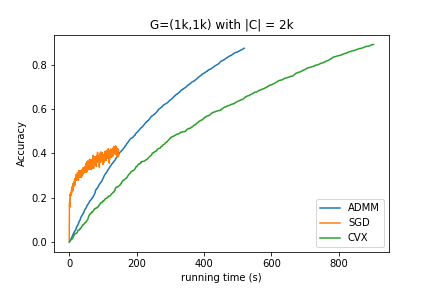
\includegraphics[scale = 0.25]{ACC_TIME_1k_1k_2k.png}
\end{figure}
\begin{figure}
    \centering
    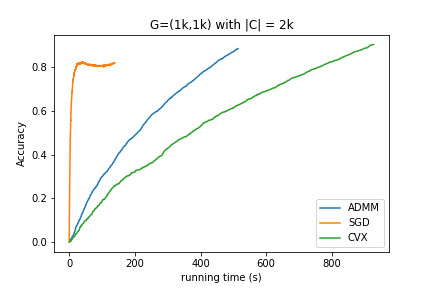
\includegraphics[scale = 0.25]{ACC_TIME_1k_1k_2k_SGD_Strong.png}
    \caption{Top : tol = $5 \times 10^{-4}$ ,Bot :tol = $5 \times 10^{-2}$}
\end{figure}
\end{columns}
\end{frame}
\begin{frame}{Results}
\begin{columns}
\column{0.5\textwidth}
\begin{figure}
    \centering
    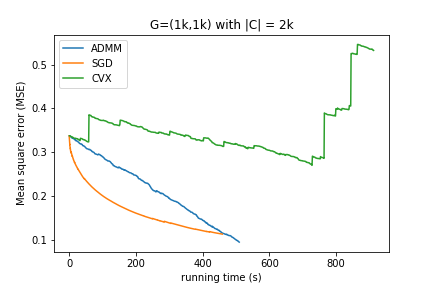
\includegraphics[scale = 0.3]{MSE_TIME_1k_1K_2k_big_iter.png}
\end{figure}
\column{0.5\textwidth}
\begin{figure}
    \centering
    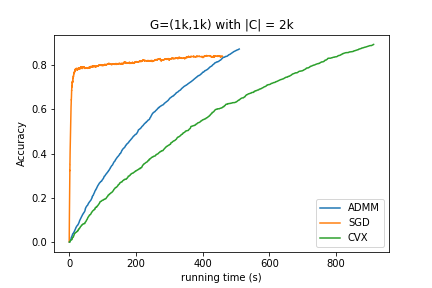
\includegraphics[scale = 0.3]{ACC_TIME_1k_1k_2k_big_iter.png}
\end{figure}
\end{columns}
\end{frame}
\section{Conclusion}
\begin{frame}[allowframebreaks]{Bibliographie}
    \bibliographystyle{plain}
    \bibliography{bibliographie}
\end{frame}
\end{document}
